\documentclass[1p]{elsarticle_modified}
%\bibliographystyle{elsarticle-num}

%\usepackage[colorlinks]{hyperref}
%\usepackage{abbrmath_seonhwa} %\Abb, \Ascr, \Acal ,\Abf, \Afrak
\usepackage{amsfonts}
\usepackage{amssymb}
\usepackage{amsmath}
\usepackage{amsthm}
\usepackage{scalefnt}
\usepackage{amsbsy}
\usepackage{kotex}
\usepackage{caption}
\usepackage{subfig}
\usepackage{color}
\usepackage{graphicx}
\usepackage{xcolor} %% white, black, red, green, blue, cyan, magenta, yellow
\usepackage{float}
\usepackage{setspace}
\usepackage{hyperref}

\usepackage{tikz}
\usetikzlibrary{arrows}

\usepackage{multirow}
\usepackage{array} % fixed length table
\usepackage{hhline}

%%%%%%%%%%%%%%%%%%%%%
\makeatletter
\renewcommand*\env@matrix[1][\arraystretch]{%
	\edef\arraystretch{#1}%
	\hskip -\arraycolsep
	\let\@ifnextchar\new@ifnextchar
	\array{*\c@MaxMatrixCols c}}
\makeatother %https://tex.stackexchange.com/questions/14071/how-can-i-increase-the-line-spacing-in-a-matrix
%%%%%%%%%%%%%%%

\usepackage[normalem]{ulem}

\newcommand{\msout}[1]{\ifmmode\text{\sout{\ensuremath{#1}}}\else\sout{#1}\fi}
%SOURCE: \msout is \stkout macro in https://tex.stackexchange.com/questions/20609/strikeout-in-math-mode

\newcommand{\cancel}[1]{
	\ifmmode
	{\color{red}\msout{#1}}
	\else
	{\color{red}\sout{#1}}
	\fi
}

\newcommand{\add}[1]{
	{\color{blue}\uwave{#1}}
}

\newcommand{\replace}[2]{
	\ifmmode
	{\color{red}\msout{#1}}{\color{blue}\uwave{#2}}
	\else
	{\color{red}\sout{#1}}{\color{blue}\uwave{#2}}
	\fi
}

\newcommand{\Sol}{\mathcal{S}} %segment
\newcommand{\D}{D} %diagram
\newcommand{\A}{\mathcal{A}} %arc


%%%%%%%%%%%%%%%%%%%%%%%%%%%%%5 test

\def\sl{\operatorname{\textup{SL}}(2,\Cbb)}
\def\psl{\operatorname{\textup{PSL}}(2,\Cbb)}
\def\quan{\mkern 1mu \triangleright \mkern 1mu}

\theoremstyle{definition}
\newtheorem{thm}{Theorem}[section]
\newtheorem{prop}[thm]{Proposition}
\newtheorem{lem}[thm]{Lemma}
\newtheorem{ques}[thm]{Question}
\newtheorem{cor}[thm]{Corollary}
\newtheorem{defn}[thm]{Definition}
\newtheorem{exam}[thm]{Example}
\newtheorem{rmk}[thm]{Remark}
\newtheorem{alg}[thm]{Algorithm}

\newcommand{\I}{\sqrt{-1}}
\begin{document}

%\begin{frontmatter}
%
%\title{Boundary parabolic representations of knots up to 8 crossings}
%
%%% Group authors per affiliation:
%\author{Yunhi Cho} 
%\address{Department of Mathematics, University of Seoul, Seoul, Korea}
%\ead{yhcho@uos.ac.kr}
%
%
%\author{Seonhwa Kim} %\fnref{s_kim}}
%\address{Center for Geometry and Physics, Institute for Basic Science, Pohang, 37673, Korea}
%\ead{ryeona17@ibs.re.kr}
%
%\author{Hyuk Kim}
%\address{Department of Mathematical Sciences, Seoul National University, Seoul 08826, Korea}
%\ead{hyukkim@snu.ac.kr}
%
%\author{Seokbeom Yoon}
%\address{Department of Mathematical Sciences, Seoul National University, Seoul, 08826,  Korea}
%\ead{sbyoon15@snu.ac.kr}
%
%\begin{abstract}
%We find all boundary parabolic representation of knots up to 8 crossings.
%
%\end{abstract}
%\begin{keyword}
%    \MSC[2010] 57M25 
%\end{keyword}
%
%\end{frontmatter}

%\linenumbers
%\tableofcontents
%
\newcommand\colored[1]{\textcolor{white}{\rule[-0.35ex]{0.8em}{1.4ex}}\kern-0.8em\color{red} #1}%
%\newcommand\colored[1]{\textcolor{white}{ #1}\kern-2.17ex	\textcolor{white}{ #1}\kern-1.81ex	\textcolor{white}{ #1}\kern-2.15ex\color{red}#1	}

{\Large $\underline{12a_{0288}~(K12a_{0288})}$}

\setlength{\tabcolsep}{10pt}
\renewcommand{\arraystretch}{1.6}
\vspace{1cm}\begin{tabular}{m{100pt}>{\centering\arraybackslash}m{274pt}}
\multirow{5}{120pt}{
	\centering
	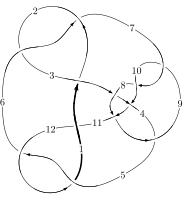
\includegraphics[width=112pt]{../../../GIT/diagram.site/Diagrams/png/1089_12a_0288.png}\\
\ \ \ A knot diagram\footnotemark}&
\allowdisplaybreaks
\textbf{Linearized knot diagam} \\
\cline{2-2}
 &
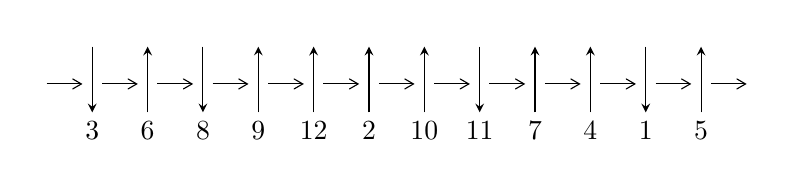
\begin{tikzpicture}[x=20pt, y=17pt]
	% nodes
	\node (C0) at (0, 0) {};
	\node (C1) at (1, 0) {};
	\node (C1U) at (1, +1) {};
	\node (C1D) at (1, -1) {3};

	\node (C2) at (2, 0) {};
	\node (C2U) at (2, +1) {};
	\node (C2D) at (2, -1) {6};

	\node (C3) at (3, 0) {};
	\node (C3U) at (3, +1) {};
	\node (C3D) at (3, -1) {8};

	\node (C4) at (4, 0) {};
	\node (C4U) at (4, +1) {};
	\node (C4D) at (4, -1) {9};

	\node (C5) at (5, 0) {};
	\node (C5U) at (5, +1) {};
	\node (C5D) at (5, -1) {12};

	\node (C6) at (6, 0) {};
	\node (C6U) at (6, +1) {};
	\node (C6D) at (6, -1) {2};

	\node (C7) at (7, 0) {};
	\node (C7U) at (7, +1) {};
	\node (C7D) at (7, -1) {10};

	\node (C8) at (8, 0) {};
	\node (C8U) at (8, +1) {};
	\node (C8D) at (8, -1) {11};

	\node (C9) at (9, 0) {};
	\node (C9U) at (9, +1) {};
	\node (C9D) at (9, -1) {7};

	\node (C10) at (10, 0) {};
	\node (C10U) at (10, +1) {};
	\node (C10D) at (10, -1) {4};

	\node (C11) at (11, 0) {};
	\node (C11U) at (11, +1) {};
	\node (C11D) at (11, -1) {1};

	\node (C12) at (12, 0) {};
	\node (C12U) at (12, +1) {};
	\node (C12D) at (12, -1) {5};
	\node (C13) at (13, 0) {};

	% arrows
	\draw[->,>={angle 60}]
	(C0) edge (C1) (C1) edge (C2) (C2) edge (C3) (C3) edge (C4) (C4) edge (C5) (C5) edge (C6) (C6) edge (C7) (C7) edge (C8) (C8) edge (C9) (C9) edge (C10) (C10) edge (C11) (C11) edge (C12) (C12) edge (C13) ;	\draw[->,>=stealth]
	(C1U) edge (C1D) (C2D) edge (C2U) (C3U) edge (C3D) (C4D) edge (C4U) (C5D) edge (C5U) (C6D) edge (C6U) (C7D) edge (C7U) (C8U) edge (C8D) (C9D) edge (C9U) (C10D) edge (C10U) (C11U) edge (C11D) (C12D) edge (C12U) ;
	\end{tikzpicture} \\
\hhline{~~} \\& 
\textbf{Solving Sequence} \\ \cline{2-2} 
 &
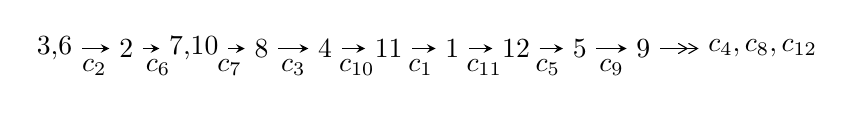
\begin{tikzpicture}[x=23pt, y=7pt]
	% node
	\node (A0) at (-1/8, 0) {3,6};
	\node (A1) at (1, 0) {2};
	\node (A2) at (33/16, 0) {7,10};
	\node (A3) at (25/8, 0) {8};
	\node (A4) at (33/8, 0) {4};
	\node (A5) at (41/8, 0) {11};
	\node (A6) at (49/8, 0) {1};
	\node (A7) at (57/8, 0) {12};
	\node (A8) at (65/8, 0) {5};
	\node (A9) at (73/8, 0) {9};
	\node (C1) at (1/2, -1) {$c_{2}$};
	\node (C2) at (3/2, -1) {$c_{6}$};
	\node (C3) at (21/8, -1) {$c_{7}$};
	\node (C4) at (29/8, -1) {$c_{3}$};
	\node (C5) at (37/8, -1) {$c_{10}$};
	\node (C6) at (45/8, -1) {$c_{1}$};
	\node (C7) at (53/8, -1) {$c_{11}$};
	\node (C8) at (61/8, -1) {$c_{5}$};
	\node (C9) at (69/8, -1) {$c_{9}$};
	\node (A10) at (11, 0) {$c_{4},c_{8},c_{12}$};

	% edge
	\draw[->,>=stealth]	
	(A0) edge (A1) (A1) edge (A2) (A2) edge (A3) (A3) edge (A4) (A4) edge (A5) (A5) edge (A6) (A6) edge (A7) (A7) edge (A8) (A8) edge (A9) ;
	\draw[->>,>={angle 60}]	
	(A9) edge (A10);
\end{tikzpicture} \\ 

\end{tabular} \\

\footnotetext{
The image of knot diagram is generated by the software ``\textbf{Draw programme}" developed by Andrew Bartholomew(\url{http://www.layer8.co.uk/maths/draw/index.htm\#Running-draw}), where we modified some parts for our purpose(\url{https://github.com/CATsTAILs/LinksPainter}).
}\phantom \\ \newline 
\centering \textbf{Ideals for irreducible components\footnotemark of $X_{\text{par}}$} 
 
\begin{align*}
I^u_{1}&=\langle 
-6.31109\times10^{21} u^{55}-7.82504\times10^{21} u^{54}+\cdots+5.87982\times10^{21} b-7.54174\times10^{21},\\
\phantom{I^u_{1}}&\phantom{= \langle  }3.46636\times10^{21} u^{55}+5.58656\times10^{21} u^{54}+\cdots+3.91988\times10^{21} a+2.03288\times10^{22},\;u^{56}+u^{55}+\cdots+5 u+1\rangle \\
I^u_{2}&=\langle 
-4.48511\times10^{91} u^{83}+8.27522\times10^{90} u^{82}+\cdots+5.10117\times10^{93} b-6.71976\times10^{93},\\
\phantom{I^u_{2}}&\phantom{= \langle  }2.37745\times10^{94} u^{83}+9.35836\times10^{93} u^{82}+\cdots+8.67198\times10^{94} a+1.23067\times10^{95},\;u^{84}+u^{83}+\cdots+88 u+17\rangle \\
I^u_{3}&=\langle 
12 a^5 u+50 a^4 u+60 a^4-58 a^3 u+200 a^3-345 a^2 u+66 a^2-132 a u+13 b-290 a+125 u-56,\\
\phantom{I^u_{3}}&\phantom{= \langle  }a^6-6 a^5 u+5 a^5-25 a^4 u-6 a^4-16 a^3 u-48 a^3+44 a^2 u-41 a^2+34 a u+20 a-4 u+11,\;u^2+1\rangle \\
I^u_{4}&=\langle 
2 b-3,\;4 a-1,\;u+1\rangle \\
\\
\end{align*}
\raggedright * 4 irreducible components of $\dim_{\mathbb{C}}=0$, with total 153 representations.\\
\footnotetext{All coefficients of polynomials are rational numbers. But the coefficients are sometimes approximated in decimal forms when there is not enough margin.}
\newpage
\renewcommand{\arraystretch}{1}
\centering \section*{I. $I^u_{1}= \langle -6.31\times10^{21} u^{55}-7.83\times10^{21} u^{54}+\cdots+5.88\times10^{21} b-7.54\times10^{21},\;3.47\times10^{21} u^{55}+5.59\times10^{21} u^{54}+\cdots+3.92\times10^{21} a+2.03\times10^{22},\;u^{56}+u^{55}+\cdots+5 u+1 \rangle$}
\flushleft \textbf{(i) Arc colorings}\\
\begin{tabular}{m{7pt} m{180pt} m{7pt} m{180pt} }
\flushright $a_{3}=$&$\begin{pmatrix}1\\0\end{pmatrix}$ \\
\flushright $a_{6}=$&$\begin{pmatrix}0\\u\end{pmatrix}$ \\
\flushright $a_{2}=$&$\begin{pmatrix}1\\u^2\end{pmatrix}$ \\
\flushright $a_{7}=$&$\begin{pmatrix}u\\u^3+u\end{pmatrix}$ \\
\flushright $a_{10}=$&$\begin{pmatrix}-0.884303 u^{55}-1.42519 u^{54}+\cdots-11.7187 u-5.18607\\1.07335 u^{55}+1.33083 u^{54}+\cdots+10.5900 u+1.28265\end{pmatrix}$ \\
\flushright $a_{8}=$&$\begin{pmatrix}0.398819 u^{55}+0.264821 u^{54}+\cdots-1.50716 u-4.14726\\-0.293268 u^{55}-0.142370 u^{54}+\cdots+7.15161 u+1.04151\end{pmatrix}$ \\
\flushright $a_{4}=$&$\begin{pmatrix}1.12125 u^{55}+0.795368 u^{54}+\cdots-1.21708 u+3.71105\\0.728912 u^{55}+0.645449 u^{54}+\cdots+5.28443 u+0.988456\end{pmatrix}$ \\
\flushright $a_{11}=$&$\begin{pmatrix}- u^4- u^2-1\\-0.0156250 u^{55}-0.0156250 u^{54}+\cdots-2.07813 u^{2}-0.0156250 u\end{pmatrix}$ \\
\flushright $a_{1}=$&$\begin{pmatrix}u^2+1\\u^2\end{pmatrix}$ \\
\flushright $a_{12}=$&$\begin{pmatrix}-1\\-0.0156250 u^{55}-0.0156250 u^{54}+\cdots-2.07813 u^{2}-0.0156250 u\end{pmatrix}$ \\
\flushright $a_{5}=$&$\begin{pmatrix}- u\\0.0156250 u^{54}+0.0156250 u^{53}+\cdots+1.07813 u+0.0156250\end{pmatrix}$ \\
\flushright $a_{9}=$&$\begin{pmatrix}-0.338735 u^{55}-0.642358 u^{54}+\cdots-7.14616 u-4.61240\\1.28465 u^{55}+1.74616 u^{54}+\cdots+13.4307 u+1.61906\end{pmatrix}$\\&\end{tabular}
\flushleft \textbf{(ii) Obstruction class $= -1$}\\~\\
\flushleft \textbf{(iii) Cusp Shapes $= -\frac{29125476928318618116311}{15679520968247263985664} u^{55}+\frac{44772161939557650505}{122496257564431749888} u^{54}+\cdots+\frac{47342986975139852519811}{1306626747353938665472} u+\frac{168360984603466865896361}{15679520968247263985664}$}\\~\\
\newpage\renewcommand{\arraystretch}{1}
\flushleft \textbf{(iv) u-Polynomials at the component}\newline \\
\begin{tabular}{m{50pt}|m{274pt}}
Crossings & \hspace{64pt}u-Polynomials at each crossing \\
\hline $$\begin{aligned}c_{1},c_{11}\end{aligned}$$&$\begin{aligned}
&u^{56}+23 u^{55}+\cdots+7 u+1
\end{aligned}$\\
\hline $$\begin{aligned}c_{2},c_{5},c_{6}\\c_{12}\end{aligned}$$&$\begin{aligned}
&u^{56}- u^{55}+\cdots-5 u+1
\end{aligned}$\\
\hline $$\begin{aligned}c_{3}\end{aligned}$$&$\begin{aligned}
&2(2 u^{56}-7 u^{55}+\cdots-1408 u+568)
\end{aligned}$\\
\hline $$\begin{aligned}c_{4}\end{aligned}$$&$\begin{aligned}
&2(2 u^{56}+5 u^{55}+\cdots-12415 u-1814)
\end{aligned}$\\
\hline $$\begin{aligned}c_{7},c_{9}\end{aligned}$$&$\begin{aligned}
&u^{56}+2 u^{55}+\cdots+111 u-16
\end{aligned}$\\
\hline $$\begin{aligned}c_{8}\end{aligned}$$&$\begin{aligned}
&u^{56}-9 u^{55}+\cdots-108 u+32
\end{aligned}$\\
\hline $$\begin{aligned}c_{10}\end{aligned}$$&$\begin{aligned}
&u^{56}-11 u^{55}+\cdots+12 u-4
\end{aligned}$\\
\hline
\end{tabular}\\~\\
\newpage\renewcommand{\arraystretch}{1}
\flushleft \textbf{(v) Riley Polynomials at the component}\newline \\
\begin{tabular}{m{50pt}|m{274pt}}
Crossings & \hspace{64pt}Riley Polynomials at each crossing \\
\hline $$\begin{aligned}c_{1},c_{11}\end{aligned}$$&$\begin{aligned}
&y^{56}+27 y^{55}+\cdots-281 y+1
\end{aligned}$\\
\hline $$\begin{aligned}c_{2},c_{5},c_{6}\\c_{12}\end{aligned}$$&$\begin{aligned}
&y^{56}+23 y^{55}+\cdots+7 y+1
\end{aligned}$\\
\hline $$\begin{aligned}c_{3}\end{aligned}$$&$\begin{aligned}
&4(4 y^{56}+203 y^{55}+\cdots+8791360 y+322624)
\end{aligned}$\\
\hline $$\begin{aligned}c_{4}\end{aligned}$$&$\begin{aligned}
&4(4 y^{56}+203 y^{55}+\cdots-6.38349\times10^{7} y+3290596)
\end{aligned}$\\
\hline $$\begin{aligned}c_{7},c_{9}\end{aligned}$$&$\begin{aligned}
&y^{56}-34 y^{55}+\cdots-3873 y+256
\end{aligned}$\\
\hline $$\begin{aligned}c_{8}\end{aligned}$$&$\begin{aligned}
&y^{56}-9 y^{55}+\cdots-14928 y+1024
\end{aligned}$\\
\hline $$\begin{aligned}c_{10}\end{aligned}$$&$\begin{aligned}
&y^{56}-13 y^{55}+\cdots-56 y+16
\end{aligned}$\\
\hline
\end{tabular}\\~\\
\newpage\flushleft \textbf{(vi) Complex Volumes and Cusp Shapes}
$$\begin{array}{c|c|c}  
\text{Solutions to }I^u_{1}& \I (\text{vol} + \sqrt{-1}CS) & \text{Cusp shape}\\
 \hline 
\begin{aligned}
u &= \phantom{-}0.641354 + 0.766924 I \\
a &= \phantom{-}0.694797 - 0.010474 I \\
b &= -0.411989 + 0.253331 I\end{aligned}
 & \phantom{-}1.69613 + 5.88626 I & \phantom{-}6.59882 - 10.04911 I \\ \hline\begin{aligned}
u &= \phantom{-}0.641354 - 0.766924 I \\
a &= \phantom{-}0.694797 + 0.010474 I \\
b &= -0.411989 - 0.253331 I\end{aligned}
 & \phantom{-}1.69613 - 5.88626 I & \phantom{-}6.59882 + 10.04911 I \\ \hline\begin{aligned}
u &= \phantom{-}0.890495 + 0.394781 I \\
a &= \phantom{-}0.56585 + 1.71637 I \\
b &= \phantom{-}0.77307 + 2.16329 I\end{aligned}
 & \phantom{-}5.23278 - 8.75525 I & \phantom{-}9.12590 + 4.28286 I \\ \hline\begin{aligned}
u &= \phantom{-}0.890495 - 0.394781 I \\
a &= \phantom{-}0.56585 - 1.71637 I \\
b &= \phantom{-}0.77307 - 2.16329 I\end{aligned}
 & \phantom{-}5.23278 + 8.75525 I & \phantom{-}9.12590 - 4.28286 I \\ \hline\begin{aligned}
u &= \phantom{-}0.680820 + 0.645893 I \\
a &= -0.27069 - 1.56272 I \\
b &= -0.429081 - 1.133110 I\end{aligned}
 & \phantom{-}5.34241 + 3.10303 I & \phantom{-}13.5555 - 6.2410 I \\ \hline\begin{aligned}
u &= \phantom{-}0.680820 - 0.645893 I \\
a &= -0.27069 + 1.56272 I \\
b &= -0.429081 + 1.133110 I\end{aligned}
 & \phantom{-}5.34241 - 3.10303 I & \phantom{-}13.5555 + 6.2410 I \\ \hline\begin{aligned}
u &= \phantom{-}0.391841 + 0.990849 I \\
a &= \phantom{-}0.108165 + 1.215430 I \\
b &= -1.272990 - 0.612251 I\end{aligned}
 & -5.11253 + 3.37715 I & -0.88601 - 5.46141 I \\ \hline\begin{aligned}
u &= \phantom{-}0.391841 - 0.990849 I \\
a &= \phantom{-}0.108165 - 1.215430 I \\
b &= -1.272990 + 0.612251 I\end{aligned}
 & -5.11253 - 3.37715 I & -0.88601 + 5.46141 I \\ \hline\begin{aligned}
u &= -0.356333 + 1.031000 I \\
a &= \phantom{-}0.112919 + 1.134410 I \\
b &= \phantom{-}1.06758 - 1.21699 I\end{aligned}
 & -3.74795 + 3.70678 I & \phantom{-}1.07262 + 1.48118 I \\ \hline\begin{aligned}
u &= -0.356333 - 1.031000 I \\
a &= \phantom{-}0.112919 - 1.134410 I \\
b &= \phantom{-}1.06758 + 1.21699 I\end{aligned}
 & -3.74795 - 3.70678 I & \phantom{-}1.07262 - 1.48118 I\\
 \hline 
 \end{array}$$\newpage$$\begin{array}{c|c|c}  
\text{Solutions to }I^u_{1}& \I (\text{vol} + \sqrt{-1}CS) & \text{Cusp shape}\\
 \hline 
\begin{aligned}
u &= -0.567758 + 0.703113 I \\
a &= -0.048537 + 0.661451 I \\
b &= \phantom{-}0.909520 + 0.756625 I\end{aligned}
 & \phantom{-}1.47606 - 2.14860 I & \phantom{-}6.53813 + 2.61588 I \\ \hline\begin{aligned}
u &= -0.567758 - 0.703113 I \\
a &= -0.048537 - 0.661451 I \\
b &= \phantom{-}0.909520 - 0.756625 I\end{aligned}
 & \phantom{-}1.47606 + 2.14860 I & \phantom{-}6.53813 - 2.61588 I \\ \hline\begin{aligned}
u &= -1.004770 + 0.465676 I \\
a &= -0.752461 + 1.121390 I \\
b &= -1.11019 + 2.22948 I\end{aligned}
 & \phantom{-}3.88963 + 0.18068 I & \phantom{-}12.1686 - 14.3132 I \\ \hline\begin{aligned}
u &= -1.004770 - 0.465676 I \\
a &= -0.752461 - 1.121390 I \\
b &= -1.11019 - 2.22948 I\end{aligned}
 & \phantom{-}3.88963 - 0.18068 I & \phantom{-}12.1686 + 14.3132 I \\ \hline\begin{aligned}
u &= \phantom{-}0.699427 + 0.539052 I \\
a &= -0.43783 - 2.08391 I \\
b &= \phantom{-}0.185339 - 1.303870 I\end{aligned}
 & \phantom{-}5.10282 - 0.74752 I & \phantom{-}13.56172 + 0.84027 I \\ \hline\begin{aligned}
u &= \phantom{-}0.699427 - 0.539052 I \\
a &= -0.43783 + 2.08391 I \\
b &= \phantom{-}0.185339 + 1.303870 I\end{aligned}
 & \phantom{-}5.10282 + 0.74752 I & \phantom{-}13.56172 - 0.84027 I \\ \hline\begin{aligned}
u &= -1.13520\phantom{ +0.000000I} \\
a &= -0.599595\phantom{ +0.000000I} \\
b &= -2.22015\phantom{ +0.000000I}\end{aligned}
 & \phantom{-}3.17493\phantom{ +0.000000I} & -46.8580\phantom{ +0.000000I} \\ \hline\begin{aligned}
u &= -0.443116 + 1.068040 I \\
a &= -0.294627 + 0.330709 I \\
b &= -0.701327 + 0.323759 I\end{aligned}
 & -6.12718 - 2.42607 I & \phantom{-0.000000 -}0. + 3.46050 I \\ \hline\begin{aligned}
u &= -0.443116 - 1.068040 I \\
a &= -0.294627 - 0.330709 I \\
b &= -0.701327 - 0.323759 I\end{aligned}
 & -6.12718 + 2.42607 I & \phantom{-0.000000 } 0. - 3.46050 I \\ \hline\begin{aligned}
u &= -0.604422 + 0.580004 I \\
a &= \phantom{-}1.67133 - 3.65644 I \\
b &= \phantom{-}0.06407 - 4.02240 I\end{aligned}
 & \phantom{-}2.96769 - 1.32540 I & -18.6606 + 10.9069 I\\
 \hline 
 \end{array}$$\newpage$$\begin{array}{c|c|c}  
\text{Solutions to }I^u_{1}& \I (\text{vol} + \sqrt{-1}CS) & \text{Cusp shape}\\
 \hline 
\begin{aligned}
u &= -0.604422 - 0.580004 I \\
a &= \phantom{-}1.67133 + 3.65644 I \\
b &= \phantom{-}0.06407 + 4.02240 I\end{aligned}
 & \phantom{-}2.96769 + 1.32540 I & -18.6606 - 10.9069 I \\ \hline\begin{aligned}
u &= \phantom{-}0.727400 + 0.390596 I \\
a &= -0.558491 - 0.668115 I \\
b &= \phantom{-}0.155223 - 0.051892 I\end{aligned}
 & \phantom{-}0.86120 - 3.19371 I & \phantom{-}6.98585 + 3.47955 I \\ \hline\begin{aligned}
u &= \phantom{-}0.727400 - 0.390596 I \\
a &= -0.558491 + 0.668115 I \\
b &= \phantom{-}0.155223 + 0.051892 I\end{aligned}
 & \phantom{-}0.86120 + 3.19371 I & \phantom{-}6.98585 - 3.47955 I \\ \hline\begin{aligned}
u &= \phantom{-}0.798907 + 0.863165 I \\
a &= \phantom{-}1.08626 + 1.62924 I \\
b &= -0.25509 + 2.32871 I\end{aligned}
 & \phantom{-}6.92651 + 10.55710 I & \phantom{-}8.79807 - 9.19219 I \\ \hline\begin{aligned}
u &= \phantom{-}0.798907 - 0.863165 I \\
a &= \phantom{-}1.08626 - 1.62924 I \\
b &= -0.25509 - 2.32871 I\end{aligned}
 & \phantom{-}6.92651 - 10.55710 I & \phantom{-}8.79807 + 9.19219 I \\ \hline\begin{aligned}
u &= -0.546311 + 1.045040 I \\
a &= -0.004162 - 0.200042 I \\
b &= -0.618017 + 0.983572 I\end{aligned}
 & -0.04707 - 3.40862 I & \phantom{-0.000000 } 0 \\ \hline\begin{aligned}
u &= -0.546311 - 1.045040 I \\
a &= -0.004162 + 0.200042 I \\
b &= -0.618017 - 0.983572 I\end{aligned}
 & -0.04707 + 3.40862 I & \phantom{-0.000000 } 0 \\ \hline\begin{aligned}
u &= \phantom{-}0.422043 + 1.122130 I \\
a &= \phantom{-}0.259194 + 0.525303 I \\
b &= \phantom{-}0.143647 - 0.242320 I\end{aligned}
 & -5.00479 + 8.23366 I & \phantom{-0.000000 } 0. - 10.38982 I \\ \hline\begin{aligned}
u &= \phantom{-}0.422043 - 1.122130 I \\
a &= \phantom{-}0.259194 - 0.525303 I \\
b &= \phantom{-}0.143647 + 0.242320 I\end{aligned}
 & -5.00479 - 8.23366 I & \phantom{-0.000000 -}0. + 10.38982 I \\ \hline\begin{aligned}
u &= \phantom{-}0.541495 + 1.089460 I \\
a &= \phantom{-}1.35077 - 1.05139 I \\
b &= \phantom{-}1.28833 + 2.18214 I\end{aligned}
 & -1.20159 + 6.69686 I & \phantom{-0.000000 } 0\\
 \hline 
 \end{array}$$\newpage$$\begin{array}{c|c|c}  
\text{Solutions to }I^u_{1}& \I (\text{vol} + \sqrt{-1}CS) & \text{Cusp shape}\\
 \hline 
\begin{aligned}
u &= \phantom{-}0.541495 - 1.089460 I \\
a &= \phantom{-}1.35077 + 1.05139 I \\
b &= \phantom{-}1.28833 - 2.18214 I\end{aligned}
 & -1.20159 - 6.69686 I & \phantom{-0.000000 } 0 \\ \hline\begin{aligned}
u &= -0.799984 + 0.939547 I \\
a &= -1.30937 + 1.40522 I \\
b &= \phantom{-}0.57203 + 2.16000 I\end{aligned}
 & \phantom{-}6.49526 - 1.44027 I & \phantom{-0.000000 } 0 \\ \hline\begin{aligned}
u &= -0.799984 - 0.939547 I \\
a &= -1.30937 - 1.40522 I \\
b &= \phantom{-}0.57203 - 2.16000 I\end{aligned}
 & \phantom{-}6.49526 + 1.44027 I & \phantom{-0.000000 } 0 \\ \hline\begin{aligned}
u &= -0.051851 + 0.762889 I \\
a &= \phantom{-}0.282476 + 1.053620 I \\
b &= -0.690965 - 0.883742 I\end{aligned}
 & -2.27089 - 5.91381 I & \phantom{-}7.94668 + 7.27969 I \\ \hline\begin{aligned}
u &= -0.051851 - 0.762889 I \\
a &= \phantom{-}0.282476 - 1.053620 I \\
b &= -0.690965 + 0.883742 I\end{aligned}
 & -2.27089 + 5.91381 I & \phantom{-}7.94668 - 7.27969 I \\ \hline\begin{aligned}
u &= -0.591203 + 1.092780 I \\
a &= \phantom{-}1.31016 - 1.25263 I \\
b &= -0.930688 - 0.609508 I\end{aligned}
 & \phantom{-}2.45649 - 6.90794 I & \phantom{-0.000000 } 0 \\ \hline\begin{aligned}
u &= -0.591203 - 1.092780 I \\
a &= \phantom{-}1.31016 + 1.25263 I \\
b &= -0.930688 + 0.609508 I\end{aligned}
 & \phantom{-}2.45649 + 6.90794 I & \phantom{-0.000000 } 0 \\ \hline\begin{aligned}
u &= \phantom{-}0.568843 + 1.123960 I \\
a &= -3.35816 - 1.22273 I \\
b &= \phantom{-}0.85524 - 3.67514 I\end{aligned}
 & -0.61428 + 8.19980 I & \phantom{-0.000000 } 0 \\ \hline\begin{aligned}
u &= \phantom{-}0.568843 - 1.123960 I \\
a &= -3.35816 + 1.22273 I \\
b &= \phantom{-}0.85524 + 3.67514 I\end{aligned}
 & -0.61428 - 8.19980 I & \phantom{-0.000000 } 0 \\ \hline\begin{aligned}
u &= -0.594804 + 1.135650 I \\
a &= \phantom{-}1.55919 - 1.02268 I \\
b &= -0.21013 - 1.56219 I\end{aligned}
 & \phantom{-}1.33863 - 10.96070 I & \phantom{-0.000000 } 0\\
 \hline 
 \end{array}$$\newpage$$\begin{array}{c|c|c}  
\text{Solutions to }I^u_{1}& \I (\text{vol} + \sqrt{-1}CS) & \text{Cusp shape}\\
 \hline 
\begin{aligned}
u &= -0.594804 - 1.135650 I \\
a &= \phantom{-}1.55919 + 1.02268 I \\
b &= -0.21013 + 1.56219 I\end{aligned}
 & \phantom{-}1.33863 + 10.96070 I & \phantom{-0.000000 } 0 \\ \hline\begin{aligned}
u &= -0.559956 + 0.434306 I \\
a &= -0.589021 - 0.157164 I \\
b &= -0.697701 + 0.414035 I\end{aligned}
 & \phantom{-}1.163170 - 0.747921 I & \phantom{-}7.34726 + 4.22076 I \\ \hline\begin{aligned}
u &= -0.559956 - 0.434306 I \\
a &= -0.589021 + 0.157164 I \\
b &= -0.697701 - 0.414035 I\end{aligned}
 & \phantom{-}1.163170 + 0.747921 I & \phantom{-}7.34726 - 4.22076 I \\ \hline\begin{aligned}
u &= \phantom{-}0.551322 + 1.170130 I \\
a &= \phantom{-}0.065982 + 0.333605 I \\
b &= -0.706084 - 0.227289 I\end{aligned}
 & -3.52575 + 8.58144 I & \phantom{-0.000000 } 0 \\ \hline\begin{aligned}
u &= \phantom{-}0.551322 - 1.170130 I \\
a &= \phantom{-}0.065982 - 0.333605 I \\
b &= -0.706084 + 0.227289 I\end{aligned}
 & -3.52575 - 8.58144 I & \phantom{-0.000000 } 0 \\ \hline\begin{aligned}
u &= \phantom{-}0.061371 + 0.690777 I \\
a &= -0.450846 + 0.828076 I \\
b &= \phantom{-}0.897751 - 0.266212 I\end{aligned}
 & -3.81337 - 0.64970 I & \phantom{-}3.11741 - 0.92674 I \\ \hline\begin{aligned}
u &= \phantom{-}0.061371 - 0.690777 I \\
a &= -0.450846 - 0.828076 I \\
b &= \phantom{-}0.897751 + 0.266212 I\end{aligned}
 & -3.81337 + 0.64970 I & \phantom{-}3.11741 + 0.92674 I \\ \hline\begin{aligned}
u &= -0.582882 + 1.176740 I \\
a &= \phantom{-}0.049432 - 0.569260 I \\
b &= \phantom{-}0.047888 - 0.543291 I\end{aligned}
 & -3.89165 - 13.47290 I & \phantom{-0.000000 } 0 \\ \hline\begin{aligned}
u &= -0.582882 - 1.176740 I \\
a &= \phantom{-}0.049432 + 0.569260 I \\
b &= \phantom{-}0.047888 + 0.543291 I\end{aligned}
 & -3.89165 + 13.47290 I & \phantom{-0.000000 } 0 \\ \hline\begin{aligned}
u &= -0.609351 + 1.211770 I \\
a &= -1.98054 + 1.28391 I \\
b &= \phantom{-}1.22737 + 2.10225 I\end{aligned}
 & \phantom{-}0.1196 - 20.0021 I & \phantom{-0.000000 } 0\\
 \hline 
 \end{array}$$\newpage$$\begin{array}{c|c|c}  
\text{Solutions to }I^u_{1}& \I (\text{vol} + \sqrt{-1}CS) & \text{Cusp shape}\\
 \hline 
\begin{aligned}
u &= -0.609351 - 1.211770 I \\
a &= -1.98054 - 1.28391 I \\
b &= \phantom{-}1.22737 - 2.10225 I\end{aligned}
 & \phantom{-}0.1196 + 20.0021 I & \phantom{-0.000000 } 0 \\ \hline\begin{aligned}
u &= \phantom{-}0.631153 + 1.210450 I \\
a &= \phantom{-}1.59641 + 1.30244 I \\
b &= -1.48858 + 1.76082 I\end{aligned}
 & -0.97220 + 12.02980 I & \phantom{-0.000000 } 0 \\ \hline\begin{aligned}
u &= \phantom{-}0.631153 - 1.210450 I \\
a &= \phantom{-}1.59641 - 1.30244 I \\
b &= -1.48858 - 1.76082 I\end{aligned}
 & -0.97220 - 12.02980 I & \phantom{-0.000000 } 0 \\ \hline\begin{aligned}
u &= -0.101342 + 0.410395 I \\
a &= -1.242190 - 0.632064 I \\
b &= \phantom{-}0.097330 + 1.042940 I\end{aligned}
 & \phantom{-}0.89200 - 1.30649 I & \phantom{-}6.20526 + 4.80910 I \\ \hline\begin{aligned}
u &= -0.101342 - 0.410395 I \\
a &= -1.242190 + 0.632064 I \\
b &= \phantom{-}0.097330 - 1.042940 I\end{aligned}
 & \phantom{-}0.89200 + 1.30649 I & \phantom{-}6.20526 - 4.80910 I \\ \hline\begin{aligned}
u &= -0.249581\phantom{ +0.000000I} \\
a &= -4.98248\phantom{ +0.000000I} \\
b &= -0.802957\phantom{ +0.000000I}\end{aligned}
 & \phantom{-}2.23670\phantom{ +0.000000I} & \phantom{-}0.606960\phantom{ +0.000000I}\\
 \hline 
 \end{array}$$\newpage\newpage\renewcommand{\arraystretch}{1}
\centering \section*{II. $I^u_{2}= \langle -4.49\times10^{91} u^{83}+8.28\times10^{90} u^{82}+\cdots+5.10\times10^{93} b-6.72\times10^{93},\;2.38\times10^{94} u^{83}+9.36\times10^{93} u^{82}+\cdots+8.67\times10^{94} a+1.23\times10^{95},\;u^{84}+u^{83}+\cdots+88 u+17 \rangle$}
\flushleft \textbf{(i) Arc colorings}\\
\begin{tabular}{m{7pt} m{180pt} m{7pt} m{180pt} }
\flushright $a_{3}=$&$\begin{pmatrix}1\\0\end{pmatrix}$ \\
\flushright $a_{6}=$&$\begin{pmatrix}0\\u\end{pmatrix}$ \\
\flushright $a_{2}=$&$\begin{pmatrix}1\\u^2\end{pmatrix}$ \\
\flushright $a_{7}=$&$\begin{pmatrix}u\\u^3+u\end{pmatrix}$ \\
\flushright $a_{10}=$&$\begin{pmatrix}-0.274153 u^{83}-0.107915 u^{82}+\cdots-4.50932 u-1.41914\\0.00879232 u^{83}-0.00162222 u^{82}+\cdots+2.60942 u+1.31730\end{pmatrix}$ \\
\flushright $a_{8}=$&$\begin{pmatrix}-0.0179921 u^{83}+0.241722 u^{82}+\cdots+45.6550 u+13.6692\\0.00995629 u^{83}+0.0822915 u^{82}+\cdots+8.95606 u+2.13864\end{pmatrix}$ \\
\flushright $a_{4}=$&$\begin{pmatrix}-0.375221 u^{83}-0.209923 u^{82}+\cdots-12.2704 u-2.30297\\-0.150797 u^{83}-0.0987334 u^{82}+\cdots-1.35636 u-0.733590\end{pmatrix}$ \\
\flushright $a_{11}=$&$\begin{pmatrix}-0.132863 u^{83}-0.0894160 u^{82}+\cdots-20.7215 u-5.84894\\-0.0224294 u^{83}-0.0235312 u^{82}+\cdots+0.893970 u+1.39768\end{pmatrix}$ \\
\flushright $a_{1}=$&$\begin{pmatrix}u^2+1\\u^2\end{pmatrix}$ \\
\flushright $a_{12}=$&$\begin{pmatrix}-0.178939 u^{83}-0.110997 u^{82}+\cdots-24.5523 u-8.40162\\1\end{pmatrix}$ \\
\flushright $a_{5}=$&$\begin{pmatrix}-0.126765 u^{83}-0.0582595 u^{82}+\cdots-18.5803 u-8.21843\\-0.0679413 u^{83}+0.000564076 u^{82}+\cdots-6.34498 u-3.04196\end{pmatrix}$ \\
\flushright $a_{9}=$&$\begin{pmatrix}-0.285202 u^{83}-0.171429 u^{82}+\cdots-9.87160 u-3.03135\\0.0104337 u^{83}-0.0117629 u^{82}+\cdots+2.05195 u+0.597007\end{pmatrix}$\\&\end{tabular}
\flushleft \textbf{(ii) Obstruction class $= -1$}\\~\\
\flushleft \textbf{(iii) Cusp Shapes $= -0.0168362 u^{83}+0.405628 u^{82}+\cdots+25.2983 u+3.62973$}\\~\\
\newpage\renewcommand{\arraystretch}{1}
\flushleft \textbf{(iv) u-Polynomials at the component}\newline \\
\begin{tabular}{m{50pt}|m{274pt}}
Crossings & \hspace{64pt}u-Polynomials at each crossing \\
\hline $$\begin{aligned}c_{1},c_{11}\end{aligned}$$&$\begin{aligned}
&u^{84}+47 u^{83}+\cdots-672 u+289
\end{aligned}$\\
\hline $$\begin{aligned}c_{2},c_{5},c_{6}\\c_{12}\end{aligned}$$&$\begin{aligned}
&u^{84}- u^{83}+\cdots-88 u+17
\end{aligned}$\\
\hline $$\begin{aligned}c_{3}\end{aligned}$$&$\begin{aligned}
&(u^{42}+u^{41}+\cdots+10 u+4)^{2}
\end{aligned}$\\
\hline $$\begin{aligned}c_{4}\end{aligned}$$&$\begin{aligned}
&(u^{42}- u^{41}+\cdots-21 u+1)^{2}
\end{aligned}$\\
\hline $$\begin{aligned}c_{7},c_{9}\end{aligned}$$&$\begin{aligned}
&(u^{42}+u^{41}+\cdots+7 u+1)^{2}
\end{aligned}$\\
\hline $$\begin{aligned}c_{8}\end{aligned}$$&$\begin{aligned}
&(u^{42}-7 u^{41}+\cdots- u+1)^{2}
\end{aligned}$\\
\hline $$\begin{aligned}c_{10}\end{aligned}$$&$\begin{aligned}
&(u^{42}+3 u^{41}+\cdots+u+1)^{2}
\end{aligned}$\\
\hline
\end{tabular}\\~\\
\newpage\renewcommand{\arraystretch}{1}
\flushleft \textbf{(v) Riley Polynomials at the component}\newline \\
\begin{tabular}{m{50pt}|m{274pt}}
Crossings & \hspace{64pt}Riley Polynomials at each crossing \\
\hline $$\begin{aligned}c_{1},c_{11}\end{aligned}$$&$\begin{aligned}
&y^{84}-21 y^{83}+\cdots-9557396 y+83521
\end{aligned}$\\
\hline $$\begin{aligned}c_{2},c_{5},c_{6}\\c_{12}\end{aligned}$$&$\begin{aligned}
&y^{84}+47 y^{83}+\cdots-672 y+289
\end{aligned}$\\
\hline $$\begin{aligned}c_{3}\end{aligned}$$&$\begin{aligned}
&(y^{42}+41 y^{41}+\cdots+308 y+16)^{2}
\end{aligned}$\\
\hline $$\begin{aligned}c_{4}\end{aligned}$$&$\begin{aligned}
&(y^{42}+33 y^{41}+\cdots-247 y+1)^{2}
\end{aligned}$\\
\hline $$\begin{aligned}c_{7},c_{9}\end{aligned}$$&$\begin{aligned}
&(y^{42}-27 y^{41}+\cdots-7 y+1)^{2}
\end{aligned}$\\
\hline $$\begin{aligned}c_{8}\end{aligned}$$&$\begin{aligned}
&(y^{42}-3 y^{41}+\cdots-7 y+1)^{2}
\end{aligned}$\\
\hline $$\begin{aligned}c_{10}\end{aligned}$$&$\begin{aligned}
&(y^{42}-7 y^{41}+\cdots-3 y+1)^{2}
\end{aligned}$\\
\hline
\end{tabular}\\~\\
\newpage\flushleft \textbf{(vi) Complex Volumes and Cusp Shapes}
$$\begin{array}{c|c|c}  
\text{Solutions to }I^u_{2}& \I (\text{vol} + \sqrt{-1}CS) & \text{Cusp shape}\\
 \hline 
\begin{aligned}
u &= -0.951872 + 0.276744 I \\
a &= -0.39157 + 1.57246 I \\
b &= -1.04779 + 2.14004 I\end{aligned}
 & \phantom{-}2.9646 + 14.3413 I & \phantom{-}4.00000 - 8.28932 I \\ \hline\begin{aligned}
u &= -0.951872 - 0.276744 I \\
a &= -0.39157 - 1.57246 I \\
b &= -1.04779 - 2.14004 I\end{aligned}
 & \phantom{-}2.9646 - 14.3413 I & \phantom{-}4.00000 + 8.28932 I \\ \hline\begin{aligned}
u &= \phantom{-}0.531874 + 0.814655 I \\
a &= -0.235436 - 0.176088 I \\
b &= \phantom{-}0.428289 + 0.678050 I\end{aligned}
 & \phantom{-}1.56120 - 1.20148 I & \phantom{-}7.68187 + 4.16647 I \\ \hline\begin{aligned}
u &= \phantom{-}0.531874 - 0.814655 I \\
a &= -0.235436 + 0.176088 I \\
b &= \phantom{-}0.428289 - 0.678050 I\end{aligned}
 & \phantom{-}1.56120 + 1.20148 I & \phantom{-}7.68187 - 4.16647 I \\ \hline\begin{aligned}
u &= \phantom{-}0.987080 + 0.316254 I \\
a &= \phantom{-}0.582224 + 1.121970 I \\
b &= \phantom{-}1.30000 + 1.90393 I\end{aligned}
 & \phantom{-}1.77491 - 6.18924 I & \phantom{-0.000000 } 0 \\ \hline\begin{aligned}
u &= \phantom{-}0.987080 - 0.316254 I \\
a &= \phantom{-}0.582224 - 1.121970 I \\
b &= \phantom{-}1.30000 - 1.90393 I\end{aligned}
 & \phantom{-}1.77491 + 6.18924 I & \phantom{-0.000000 } 0 \\ \hline\begin{aligned}
u &= -0.472668 + 0.925828 I \\
a &= -1.38938 - 0.57724 I \\
b &= -0.85123 + 1.67366 I\end{aligned}
 & \phantom{-}0.88637 - 2.06372 I & \phantom{-0.000000 } 0 \\ \hline\begin{aligned}
u &= -0.472668 - 0.925828 I \\
a &= -1.38938 + 0.57724 I \\
b &= -0.85123 - 1.67366 I\end{aligned}
 & \phantom{-}0.88637 + 2.06372 I & \phantom{-0.000000 } 0 \\ \hline\begin{aligned}
u &= -0.365634 + 0.990499 I \\
a &= \phantom{-}2.37994 - 2.01802 I \\
b &= -0.146160 - 1.186050 I\end{aligned}
 & -1.39551 - 2.76342 I & \phantom{-0.000000 } 0 \\ \hline\begin{aligned}
u &= -0.365634 - 0.990499 I \\
a &= \phantom{-}2.37994 + 2.01802 I \\
b &= -0.146160 + 1.186050 I\end{aligned}
 & -1.39551 + 2.76342 I & \phantom{-0.000000 } 0\\
 \hline 
 \end{array}$$\newpage$$\begin{array}{c|c|c}  
\text{Solutions to }I^u_{2}& \I (\text{vol} + \sqrt{-1}CS) & \text{Cusp shape}\\
 \hline 
\begin{aligned}
u &= \phantom{-}0.166361 + 1.064190 I \\
a &= \phantom{-}0.222499 + 0.775256 I \\
b &= \phantom{-}0.501062 - 0.154481 I\end{aligned}
 & -3.70167 - 1.01542 I & \phantom{-0.000000 } 0 \\ \hline\begin{aligned}
u &= \phantom{-}0.166361 - 1.064190 I \\
a &= \phantom{-}0.222499 - 0.775256 I \\
b &= \phantom{-}0.501062 + 0.154481 I\end{aligned}
 & -3.70167 + 1.01542 I & \phantom{-0.000000 } 0 \\ \hline\begin{aligned}
u &= -0.861223 + 0.274631 I \\
a &= \phantom{-}0.447664 - 0.841230 I \\
b &= -0.101282 - 0.359060 I\end{aligned}
 & -1.20076 + 8.16087 I & \phantom{-}3.94706 - 7.65229 I \\ \hline\begin{aligned}
u &= -0.861223 - 0.274631 I \\
a &= \phantom{-}0.447664 + 0.841230 I \\
b &= -0.101282 + 0.359060 I\end{aligned}
 & -1.20076 - 8.16087 I & \phantom{-}3.94706 + 7.65229 I \\ \hline\begin{aligned}
u &= -0.219257 + 0.874467 I \\
a &= \phantom{-}3.40559 - 2.71073 I \\
b &= \phantom{-}0.020182 - 0.631523 I\end{aligned}
 & -0.621946 + 0.257129 I & \phantom{-}8.13768 + 2.68186 I \\ \hline\begin{aligned}
u &= -0.219257 - 0.874467 I \\
a &= \phantom{-}3.40559 + 2.71073 I \\
b &= \phantom{-}0.020182 + 0.631523 I\end{aligned}
 & -0.621946 - 0.257129 I & \phantom{-}8.13768 - 2.68186 I \\ \hline\begin{aligned}
u &= \phantom{-}0.307330 + 1.066780 I \\
a &= -5.67618 - 0.22144 I \\
b &= \phantom{-}0.08332 - 2.91001 I\end{aligned}
 & -2.80543 + 0.38762 I & \phantom{-0.000000 } 0 \\ \hline\begin{aligned}
u &= \phantom{-}0.307330 - 1.066780 I \\
a &= -5.67618 + 0.22144 I \\
b &= \phantom{-}0.08332 + 2.91001 I\end{aligned}
 & -2.80543 - 0.38762 I & \phantom{-0.000000 } 0 \\ \hline\begin{aligned}
u &= -0.816869 + 0.351666 I \\
a &= \phantom{-}0.02403 - 1.83361 I \\
b &= \phantom{-}0.05111 - 1.46523 I\end{aligned}
 & \phantom{-}3.66382 + 5.70185 I & \phantom{-}10.61456 - 6.99288 I \\ \hline\begin{aligned}
u &= -0.816869 - 0.351666 I \\
a &= \phantom{-}0.02403 + 1.83361 I \\
b &= \phantom{-}0.05111 + 1.46523 I\end{aligned}
 & \phantom{-}3.66382 - 5.70185 I & \phantom{-}10.61456 + 6.99288 I\\
 \hline 
 \end{array}$$\newpage$$\begin{array}{c|c|c}  
\text{Solutions to }I^u_{2}& \I (\text{vol} + \sqrt{-1}CS) & \text{Cusp shape}\\
 \hline 
\begin{aligned}
u &= \phantom{-}0.585604 + 0.948707 I \\
a &= -1.32890 - 1.58654 I \\
b &= \phantom{-}0.668874 - 0.815038 I\end{aligned}
 & \phantom{-}4.44406 + 1.79873 I & \phantom{-0.000000 } 0 \\ \hline\begin{aligned}
u &= \phantom{-}0.585604 - 0.948707 I \\
a &= -1.32890 + 1.58654 I \\
b &= \phantom{-}0.668874 + 0.815038 I\end{aligned}
 & \phantom{-}4.44406 - 1.79873 I & \phantom{-0.000000 } 0 \\ \hline\begin{aligned}
u &= -0.855194 + 0.715858 I \\
a &= -0.76816 + 1.52285 I \\
b &= -0.13960 + 2.24229 I\end{aligned}
 & \phantom{-}7.14323 - 4.60033 I & \phantom{-0.000000 } 0 \\ \hline\begin{aligned}
u &= -0.855194 - 0.715858 I \\
a &= -0.76816 - 1.52285 I \\
b &= -0.13960 - 2.24229 I\end{aligned}
 & \phantom{-}7.14323 + 4.60033 I & \phantom{-0.000000 } 0 \\ \hline\begin{aligned}
u &= \phantom{-}0.568046 + 0.959810 I \\
a &= \phantom{-}1.37749 + 1.72915 I \\
b &= -0.76692 + 1.63638 I\end{aligned}
 & -4.13754 + 2.24209 I & \phantom{-0.000000 } 0 \\ \hline\begin{aligned}
u &= \phantom{-}0.568046 - 0.959810 I \\
a &= \phantom{-}1.37749 - 1.72915 I \\
b &= -0.76692 - 1.63638 I\end{aligned}
 & -4.13754 - 2.24209 I & \phantom{-0.000000 } 0 \\ \hline\begin{aligned}
u &= -0.758844 + 0.419717 I \\
a &= -0.287572 - 1.117020 I \\
b &= \phantom{-}0.668874 - 0.815038 I\end{aligned}
 & \phantom{-}4.44406 + 1.79873 I & \phantom{-}12.47510 - 0.83291 I \\ \hline\begin{aligned}
u &= -0.758844 - 0.419717 I \\
a &= -0.287572 + 1.117020 I \\
b &= \phantom{-}0.668874 + 0.815038 I\end{aligned}
 & \phantom{-}4.44406 - 1.79873 I & \phantom{-}12.47510 + 0.83291 I \\ \hline\begin{aligned}
u &= -0.537381 + 1.003410 I \\
a &= \phantom{-}3.69954 - 1.88396 I \\
b &= -0.46119 - 3.74468 I\end{aligned}
 & \phantom{-}1.69916 - 3.19900 I & \phantom{-0.000000 } 0 \\ \hline\begin{aligned}
u &= -0.537381 - 1.003410 I \\
a &= \phantom{-}3.69954 + 1.88396 I \\
b &= -0.46119 + 3.74468 I\end{aligned}
 & \phantom{-}1.69916 + 3.19900 I & \phantom{-0.000000 } 0\\
 \hline 
 \end{array}$$\newpage$$\begin{array}{c|c|c}  
\text{Solutions to }I^u_{2}& \I (\text{vol} + \sqrt{-1}CS) & \text{Cusp shape}\\
 \hline 
\begin{aligned}
u &= \phantom{-}0.826710 + 0.792492 I \\
a &= \phantom{-}1.19449 + 1.56505 I \\
b &= -0.13960 + 2.24229 I\end{aligned}
 & \phantom{-}7.14323 - 4.60033 I & \phantom{-0.000000 } 0 \\ \hline\begin{aligned}
u &= \phantom{-}0.826710 - 0.792492 I \\
a &= \phantom{-}1.19449 - 1.56505 I \\
b &= -0.13960 - 2.24229 I\end{aligned}
 & \phantom{-}7.14323 + 4.60033 I & \phantom{-0.000000 } 0 \\ \hline\begin{aligned}
u &= -0.093008 + 1.146880 I \\
a &= \phantom{-}1.30559 + 0.60076 I \\
b &= \phantom{-}0.020182 + 0.631523 I\end{aligned}
 & -0.621946 - 0.257129 I & \phantom{-0.000000 } 0 \\ \hline\begin{aligned}
u &= -0.093008 - 1.146880 I \\
a &= \phantom{-}1.30559 - 0.60076 I \\
b &= \phantom{-}0.020182 - 0.631523 I\end{aligned}
 & -0.621946 + 0.257129 I & \phantom{-0.000000 } 0 \\ \hline\begin{aligned}
u &= -0.441120 + 1.073580 I \\
a &= -0.313016 - 0.998766 I \\
b &= -0.145380 - 0.195788 I\end{aligned}
 & -6.13332 - 4.53919 I & \phantom{-0.000000 } 0 \\ \hline\begin{aligned}
u &= -0.441120 - 1.073580 I \\
a &= -0.313016 + 0.998766 I \\
b &= -0.145380 + 0.195788 I\end{aligned}
 & -6.13332 + 4.53919 I & \phantom{-0.000000 } 0 \\ \hline\begin{aligned}
u &= \phantom{-}0.015777 + 1.168210 I \\
a &= \phantom{-}0.254753 + 1.283830 I \\
b &= \phantom{-}0.259413 - 0.533713 I\end{aligned}
 & -3.54870 - 1.34243 I & \phantom{-0.000000 } 0 \\ \hline\begin{aligned}
u &= \phantom{-}0.015777 - 1.168210 I \\
a &= \phantom{-}0.254753 - 1.283830 I \\
b &= \phantom{-}0.259413 + 0.533713 I\end{aligned}
 & -3.54870 + 1.34243 I & \phantom{-0.000000 } 0 \\ \hline\begin{aligned}
u &= \phantom{-}0.246543 + 1.147790 I \\
a &= \phantom{-}2.96006 - 1.66756 I \\
b &= \phantom{-}0.08332 + 2.91001 I\end{aligned}
 & -2.80543 - 0.38762 I & \phantom{-0.000000 } 0 \\ \hline\begin{aligned}
u &= \phantom{-}0.246543 - 1.147790 I \\
a &= \phantom{-}2.96006 + 1.66756 I \\
b &= \phantom{-}0.08332 - 2.91001 I\end{aligned}
 & -2.80543 + 0.38762 I & \phantom{-0.000000 } 0\\
 \hline 
 \end{array}$$\newpage$$\begin{array}{c|c|c}  
\text{Solutions to }I^u_{2}& \I (\text{vol} + \sqrt{-1}CS) & \text{Cusp shape}\\
 \hline 
\begin{aligned}
u &= \phantom{-}0.790539 + 0.233655 I \\
a &= \phantom{-}0.254852 - 0.304931 I \\
b &= \phantom{-}0.744215 - 0.026824 I\end{aligned}
 & -0.77775 - 3.57467 I & \phantom{-}2.99358 + 1.46864 I \\ \hline\begin{aligned}
u &= \phantom{-}0.790539 - 0.233655 I \\
a &= \phantom{-}0.254852 + 0.304931 I \\
b &= \phantom{-}0.744215 + 0.026824 I\end{aligned}
 & -0.77775 + 3.57467 I & \phantom{-}2.99358 - 1.46864 I \\ \hline\begin{aligned}
u &= \phantom{-}0.753325 + 0.332759 I \\
a &= -0.52004 - 2.83483 I \\
b &= -0.46119 - 3.74468 I\end{aligned}
 & \phantom{-}1.69916 - 3.19900 I & -4.91732 - 10.84472 I \\ \hline\begin{aligned}
u &= \phantom{-}0.753325 - 0.332759 I \\
a &= -0.52004 + 2.83483 I \\
b &= -0.46119 + 3.74468 I\end{aligned}
 & \phantom{-}1.69916 + 3.19900 I & -4.91732 + 10.84472 I \\ \hline\begin{aligned}
u &= \phantom{-}0.587978 + 1.024140 I \\
a &= -1.45243 - 1.33342 I \\
b &= \phantom{-}0.05111 - 1.46523 I\end{aligned}
 & \phantom{-}3.66382 + 5.70185 I & \phantom{-0.000000 } 0 \\ \hline\begin{aligned}
u &= \phantom{-}0.587978 - 1.024140 I \\
a &= -1.45243 + 1.33342 I \\
b &= \phantom{-}0.05111 + 1.46523 I\end{aligned}
 & \phantom{-}3.66382 - 5.70185 I & \phantom{-0.000000 } 0 \\ \hline\begin{aligned}
u &= -0.537462 + 1.060840 I \\
a &= -2.06677 + 1.86366 I \\
b &= \phantom{-}0.87584 + 1.89908 I\end{aligned}
 & -2.44680 - 10.28750 I & \phantom{-0.000000 } 0 \\ \hline\begin{aligned}
u &= -0.537462 - 1.060840 I \\
a &= -2.06677 - 1.86366 I \\
b &= \phantom{-}0.87584 - 1.89908 I\end{aligned}
 & -2.44680 + 10.28750 I & \phantom{-0.000000 } 0 \\ \hline\begin{aligned}
u &= -0.620482 + 0.509254 I \\
a &= -0.955022 + 0.401385 I \\
b &= \phantom{-}0.428289 + 0.678050 I\end{aligned}
 & \phantom{-}1.56120 - 1.20148 I & \phantom{-}7.68187 + 4.16647 I \\ \hline\begin{aligned}
u &= -0.620482 - 0.509254 I \\
a &= -0.955022 - 0.401385 I \\
b &= \phantom{-}0.428289 - 0.678050 I\end{aligned}
 & \phantom{-}1.56120 + 1.20148 I & \phantom{-}7.68187 - 4.16647 I\\
 \hline 
 \end{array}$$\newpage$$\begin{array}{c|c|c}  
\text{Solutions to }I^u_{2}& \I (\text{vol} + \sqrt{-1}CS) & \text{Cusp shape}\\
 \hline 
\begin{aligned}
u &= -0.510672 + 1.083630 I \\
a &= -0.114052 + 0.483358 I \\
b &= \phantom{-}0.744215 - 0.026824 I\end{aligned}
 & -0.77775 - 3.57467 I & \phantom{-0.000000 } 0 \\ \hline\begin{aligned}
u &= -0.510672 - 1.083630 I \\
a &= -0.114052 - 0.483358 I \\
b &= \phantom{-}0.744215 + 0.026824 I\end{aligned}
 & -0.77775 + 3.57467 I & \phantom{-0.000000 } 0 \\ \hline\begin{aligned}
u &= -0.197785 + 1.208910 I \\
a &= -0.388972 + 0.092186 I \\
b &= -0.146160 + 1.186050 I\end{aligned}
 & -1.39551 + 2.76342 I & \phantom{-0.000000 } 0 \\ \hline\begin{aligned}
u &= -0.197785 - 1.208910 I \\
a &= -0.388972 - 0.092186 I \\
b &= -0.146160 - 1.186050 I\end{aligned}
 & -1.39551 - 2.76342 I & \phantom{-0.000000 } 0 \\ \hline\begin{aligned}
u &= \phantom{-}0.358263 + 1.176890 I \\
a &= \phantom{-}0.438284 + 0.625720 I \\
b &= -0.576547\phantom{ +0.000000I}\end{aligned}
 & -4.99175\phantom{ +0.000000I} & \phantom{-0.000000 } 0 \\ \hline\begin{aligned}
u &= \phantom{-}0.358263 - 1.176890 I \\
a &= \phantom{-}0.438284 - 0.625720 I \\
b &= -0.576547\phantom{ +0.000000I}\end{aligned}
 & -4.99175\phantom{ +0.000000I} & \phantom{-0.000000 } 0 \\ \hline\begin{aligned}
u &= \phantom{-}0.574474 + 1.095730 I \\
a &= \phantom{-}0.156893 - 0.575244 I \\
b &= -0.101282 - 0.359060 I\end{aligned}
 & -1.20076 + 8.16087 I & \phantom{-0.000000 } 0 \\ \hline\begin{aligned}
u &= \phantom{-}0.574474 - 1.095730 I \\
a &= \phantom{-}0.156893 + 0.575244 I \\
b &= -0.101282 + 0.359060 I\end{aligned}
 & -1.20076 - 8.16087 I & \phantom{-0.000000 } 0 \\ \hline\begin{aligned}
u &= -0.578971 + 0.461942 I \\
a &= -0.82324 + 2.49340 I \\
b &= -0.47444 + 1.70352 I\end{aligned}
 & -0.66943 + 5.77796 I & \phantom{-}4.70723 - 3.77194 I \\ \hline\begin{aligned}
u &= -0.578971 - 0.461942 I \\
a &= -0.82324 - 2.49340 I \\
b &= -0.47444 - 1.70352 I\end{aligned}
 & -0.66943 - 5.77796 I & \phantom{-}4.70723 + 3.77194 I\\
 \hline 
 \end{array}$$\newpage$$\begin{array}{c|c|c}  
\text{Solutions to }I^u_{2}& \I (\text{vol} + \sqrt{-1}CS) & \text{Cusp shape}\\
 \hline 
\begin{aligned}
u &= \phantom{-}0.716730 + 0.176249 I \\
a &= -0.540642 + 0.599446 I \\
b &= \phantom{-}0.379962 + 0.861183 I\end{aligned}
 & -1.62437 + 4.60168 I & \phantom{-}1.92175 - 9.10658 I \\ \hline\begin{aligned}
u &= \phantom{-}0.716730 - 0.176249 I \\
a &= -0.540642 - 0.599446 I \\
b &= \phantom{-}0.379962 - 0.861183 I\end{aligned}
 & -1.62437 - 4.60168 I & \phantom{-}1.92175 + 9.10658 I \\ \hline\begin{aligned}
u &= \phantom{-}0.633608 + 0.363234 I \\
a &= \phantom{-}0.414127 + 0.949449 I \\
b &= -0.85123 + 1.67366 I\end{aligned}
 & \phantom{-}0.88637 - 2.06372 I & \phantom{-}7.58768 + 6.20553 I \\ \hline\begin{aligned}
u &= \phantom{-}0.633608 - 0.363234 I \\
a &= \phantom{-}0.414127 - 0.949449 I \\
b &= -0.85123 - 1.67366 I\end{aligned}
 & \phantom{-}0.88637 + 2.06372 I & \phantom{-}7.58768 - 6.20553 I \\ \hline\begin{aligned}
u &= -0.277378 + 1.257970 I \\
a &= -0.335234 + 0.865928 I \\
b &= \phantom{-}0.379962 - 0.861183 I\end{aligned}
 & -1.62437 - 4.60168 I & \phantom{-0.000000 } 0 \\ \hline\begin{aligned}
u &= -0.277378 - 1.257970 I \\
a &= -0.335234 - 0.865928 I \\
b &= \phantom{-}0.379962 + 0.861183 I\end{aligned}
 & -1.62437 + 4.60168 I & \phantom{-0.000000 } 0 \\ \hline\begin{aligned}
u &= -0.270661 + 1.259850 I \\
a &= -0.593163 + 0.562481 I \\
b &= -0.145380 + 0.195788 I\end{aligned}
 & -6.13332 + 4.53919 I & \phantom{-0.000000 } 0 \\ \hline\begin{aligned}
u &= -0.270661 - 1.259850 I \\
a &= -0.593163 - 0.562481 I \\
b &= -0.145380 - 0.195788 I\end{aligned}
 & -6.13332 - 4.53919 I & \phantom{-0.000000 } 0 \\ \hline\begin{aligned}
u &= \phantom{-}0.100542 + 1.292600 I \\
a &= -0.145253 + 1.056930 I \\
b &= -0.47444 - 1.70352 I\end{aligned}
 & -0.66943 - 5.77796 I & \phantom{-0.000000 } 0 \\ \hline\begin{aligned}
u &= \phantom{-}0.100542 - 1.292600 I \\
a &= -0.145253 - 1.056930 I \\
b &= -0.47444 + 1.70352 I\end{aligned}
 & -0.66943 + 5.77796 I & \phantom{-0.000000 } 0\\
 \hline 
 \end{array}$$\newpage$$\begin{array}{c|c|c}  
\text{Solutions to }I^u_{2}& \I (\text{vol} + \sqrt{-1}CS) & \text{Cusp shape}\\
 \hline 
\begin{aligned}
u &= \phantom{-}0.629938 + 1.144520 I \\
a &= \phantom{-}1.88349 + 1.45771 I \\
b &= -1.04779 + 2.14004 I\end{aligned}
 & \phantom{-}2.9646 + 14.3413 I & \phantom{-0.000000 } 0 \\ \hline\begin{aligned}
u &= \phantom{-}0.629938 - 1.144520 I \\
a &= \phantom{-}1.88349 - 1.45771 I \\
b &= -1.04779 - 2.14004 I\end{aligned}
 & \phantom{-}2.9646 - 14.3413 I & \phantom{-0.000000 } 0 \\ \hline\begin{aligned}
u &= \phantom{-}0.425157 + 1.241880 I \\
a &= \phantom{-}0.709496 + 0.661172 I \\
b &= -0.780021\phantom{ +0.000000I}\end{aligned}
 & -4.89562\phantom{ +0.000000I} & \phantom{-0.000000 } 0 \\ \hline\begin{aligned}
u &= \phantom{-}0.425157 - 1.241880 I \\
a &= \phantom{-}0.709496 - 0.661172 I \\
b &= -0.780021\phantom{ +0.000000I}\end{aligned}
 & -4.89562\phantom{ +0.000000I} & \phantom{-0.000000 } 0 \\ \hline\begin{aligned}
u &= \phantom{-}0.164634 + 0.664229 I \\
a &= \phantom{-}1.79299 + 0.74893 I \\
b &= \phantom{-}0.259413 + 0.533713 I\end{aligned}
 & -3.54870 + 1.34243 I & \phantom{-}1.03679 - 4.26706 I \\ \hline\begin{aligned}
u &= \phantom{-}0.164634 - 0.664229 I \\
a &= \phantom{-}1.79299 - 0.74893 I \\
b &= \phantom{-}0.259413 - 0.533713 I\end{aligned}
 & -3.54870 - 1.34243 I & \phantom{-}1.03679 + 4.26706 I \\ \hline\begin{aligned}
u &= -0.673733 + 1.141180 I \\
a &= -1.49035 + 1.37377 I \\
b &= \phantom{-}1.30000 + 1.90393 I\end{aligned}
 & \phantom{-}1.77491 - 6.18924 I & \phantom{-0.000000 } 0 \\ \hline\begin{aligned}
u &= -0.673733 - 1.141180 I \\
a &= -1.49035 - 1.37377 I \\
b &= \phantom{-}1.30000 - 1.90393 I\end{aligned}
 & \phantom{-}1.77491 + 6.18924 I & \phantom{-0.000000 } 0 \\ \hline\begin{aligned}
u &= -0.260548 + 1.338350 I \\
a &= \phantom{-}0.141594 + 1.088570 I \\
b &= \phantom{-}0.87584 - 1.89908 I\end{aligned}
 & -2.44680 + 10.28750 I & \phantom{-0.000000 } 0 \\ \hline\begin{aligned}
u &= -0.260548 - 1.338350 I \\
a &= \phantom{-}0.141594 - 1.088570 I \\
b &= \phantom{-}0.87584 + 1.89908 I\end{aligned}
 & -2.44680 - 10.28750 I & \phantom{-0.000000 } 0\\
 \hline 
 \end{array}$$\newpage$$\begin{array}{c|c|c}  
\text{Solutions to }I^u_{2}& \I (\text{vol} + \sqrt{-1}CS) & \text{Cusp shape}\\
 \hline 
\begin{aligned}
u &= \phantom{-}0.182393 + 1.356620 I \\
a &= \phantom{-}0.071105 + 1.273620 I \\
b &= -0.76692 - 1.63638 I\end{aligned}
 & -4.13754 - 2.24209 I & \phantom{-0.000000 } 0 \\ \hline\begin{aligned}
u &= \phantom{-}0.182393 - 1.356620 I \\
a &= \phantom{-}0.071105 - 1.273620 I \\
b &= -0.76692 + 1.63638 I\end{aligned}
 & -4.13754 + 2.24209 I & \phantom{-0.000000 } 0 \\ \hline\begin{aligned}
u &= -0.352141 + 0.038419 I \\
a &= \phantom{-}1.45162 - 1.80927 I \\
b &= \phantom{-}0.501062 + 0.154481 I\end{aligned}
 & -3.70167 + 1.01542 I & \phantom{-}0.525020 - 1.212964 I \\ \hline\begin{aligned}
u &= -0.352141 - 0.038419 I \\
a &= \phantom{-}1.45162 + 1.80927 I \\
b &= \phantom{-}0.501062 - 0.154481 I\end{aligned}
 & -3.70167 - 1.01542 I & \phantom{-}0.525020 + 1.212964 I\\
 \hline 
 \end{array}$$\newpage\newpage\renewcommand{\arraystretch}{1}
\centering \section*{III. $I^u_{3}= \langle 12 a^5 u+50 a^4 u+\cdots-290 a-56,\;-6 a^5 u-25 a^4 u+\cdots+20 a+11,\;u^2+1 \rangle$}
\flushleft \textbf{(i) Arc colorings}\\
\begin{tabular}{m{7pt} m{180pt} m{7pt} m{180pt} }
\flushright $a_{3}=$&$\begin{pmatrix}1\\0\end{pmatrix}$ \\
\flushright $a_{6}=$&$\begin{pmatrix}0\\u\end{pmatrix}$ \\
\flushright $a_{2}=$&$\begin{pmatrix}1\\-1\end{pmatrix}$ \\
\flushright $a_{7}=$&$\begin{pmatrix}u\\0\end{pmatrix}$ \\
\flushright $a_{10}=$&$\begin{pmatrix}a\\-0.923077 a^{5} u-3.84615 a^{4} u+\cdots+22.3077 a+4.30769\end{pmatrix}$ \\
\flushright $a_{8}=$&$\begin{pmatrix}-0.923077 a^{5} u-7.69231 a^{4} u+\cdots+8.84615 a+10.1538\\0.615385 a^{5} u+2.23077 a^{4} u+\cdots-17.5385 a-1.53846\end{pmatrix}$ \\
\flushright $a_{4}=$&$\begin{pmatrix}0.307692 a^{5} u+5.84615 a^{4} u+\cdots+7.53846 a-8\\-3.46154 a^{4} u-13.5385 a^{3} u+\cdots-13.6154 a+2.46154\end{pmatrix}$ \\
\flushright $a_{11}=$&$\begin{pmatrix}-1\\-2.30769 a^{5} u-10.6154 a^{4} u+\cdots+42.7692 a+15.7692\end{pmatrix}$ \\
\flushright $a_{1}=$&$\begin{pmatrix}0\\-1\end{pmatrix}$ \\
\flushright $a_{12}=$&$\begin{pmatrix}-1\\-2.30769 a^{5} u-10.6154 a^{4} u+\cdots+42.7692 a+14.7692\end{pmatrix}$ \\
\flushright $a_{5}=$&$\begin{pmatrix}- u\\-11.5385 a^{4} u-42.4615 a^{3} u+\cdots-40.3846 a+13.5385\end{pmatrix}$ \\
\flushright $a_{9}=$&$\begin{pmatrix}-0.923077 a^{5} u-3.84615 a^{4} u+\cdots+23.3077 a+4.30769\\-0.923077 a^{5} u-3.84615 a^{4} u+\cdots+22.3077 a+4.30769\end{pmatrix}$\\&\end{tabular}
\flushleft \textbf{(ii) Obstruction class $= 1$}\\~\\
\flushleft \textbf{(iii) Cusp Shapes $= \frac{20}{13} a^5-\frac{100}{13} a^4 u+\frac{92}{13} a^4-\frac{368}{13} a^3 u-\frac{36}{13} a^3-\frac{292}{13} a^2 u-\frac{484}{13} a^2+\frac{232}{13} a u-\frac{324}{13} a+\frac{76}{13} u-\frac{4}{13}$}\\~\\
\newpage\renewcommand{\arraystretch}{1}
\flushleft \textbf{(iv) u-Polynomials at the component}\newline \\
\begin{tabular}{m{50pt}|m{274pt}}
Crossings & \hspace{64pt}u-Polynomials at each crossing \\
\hline $$\begin{aligned}c_{1},c_{11}\end{aligned}$$&$\begin{aligned}
&(u-1)^{12}
\end{aligned}$\\
\hline $$\begin{aligned}c_{2},c_{5},c_{6}\\c_{12}\end{aligned}$$&$\begin{aligned}
&(u^2+1)^6
\end{aligned}$\\
\hline $$\begin{aligned}c_{3},c_{10}\end{aligned}$$&$\begin{aligned}
&u^{12}- u^{10}+5 u^8+6 u^4-3 u^2+1
\end{aligned}$\\
\hline $$\begin{aligned}c_{4}\end{aligned}$$&$\begin{aligned}
&u^{12}+3 u^{10}+5 u^8+4 u^6+2 u^4+u^2+1
\end{aligned}$\\
\hline $$\begin{aligned}c_{7}\end{aligned}$$&$\begin{aligned}
&(u^6- u^5- u^4+2 u^3- u+1)^2
\end{aligned}$\\
\hline $$\begin{aligned}c_{8},c_{9}\end{aligned}$$&$\begin{aligned}
&(u^6+u^5- u^4-2 u^3+u+1)^2
\end{aligned}$\\
\hline
\end{tabular}\\~\\
\newpage\renewcommand{\arraystretch}{1}
\flushleft \textbf{(v) Riley Polynomials at the component}\newline \\
\begin{tabular}{m{50pt}|m{274pt}}
Crossings & \hspace{64pt}Riley Polynomials at each crossing \\
\hline $$\begin{aligned}c_{1},c_{11}\end{aligned}$$&$\begin{aligned}
&(y-1)^{12}
\end{aligned}$\\
\hline $$\begin{aligned}c_{2},c_{5},c_{6}\\c_{12}\end{aligned}$$&$\begin{aligned}
&(y+1)^{12}
\end{aligned}$\\
\hline $$\begin{aligned}c_{3},c_{10}\end{aligned}$$&$\begin{aligned}
&(y^6- y^5+5 y^4+6 y^2-3 y+1)^2
\end{aligned}$\\
\hline $$\begin{aligned}c_{4}\end{aligned}$$&$\begin{aligned}
&(y^6+3 y^5+5 y^4+4 y^3+2 y^2+y+1)^2
\end{aligned}$\\
\hline $$\begin{aligned}c_{7},c_{8},c_{9}\end{aligned}$$&$\begin{aligned}
&(y^6-3 y^5+5 y^4-4 y^3+2 y^2- y+1)^2
\end{aligned}$\\
\hline
\end{tabular}\\~\\
\newpage\flushleft \textbf{(vi) Complex Volumes and Cusp Shapes}
$$\begin{array}{c|c|c}  
\text{Solutions to }I^u_{3}& \I (\text{vol} + \sqrt{-1}CS) & \text{Cusp shape}\\
 \hline 
\begin{aligned}
u &= \phantom{-0.000000 -}1.000000 I \\
a &= -0.655968 + 0.901719 I \\
b &= -0.664531 - 0.428243 I\end{aligned}
 & -5.18047 + 0.92430 I & -5.71672 - 0.79423 I \\ \hline\begin{aligned}
u &= \phantom{-0.000000 -}1.000000 I \\
a &= \phantom{-}0.415113 + 0.618748 I \\
b &= \phantom{-}0.558752 - 1.073950 I\end{aligned}
 & -3.28987 + 5.69302 I & -2.00000 - 5.51057 I \\ \hline\begin{aligned}
u &= \phantom{-0.000000 -}1.000000 I \\
a &= -0.655968 + 1.098280 I \\
b &= \phantom{-}0.664531 - 0.428243 I\end{aligned}
 & -5.18047 - 0.92430 I & -5.71672 + 0.79423 I \\ \hline\begin{aligned}
u &= \phantom{-0.000000 -}1.000000 I \\
a &= \phantom{-}0.41511 + 1.38125 I \\
b &= -0.558752 - 1.073950 I\end{aligned}
 & -3.28987 - 5.69302 I & -2.00000 + 5.51057 I \\ \hline\begin{aligned}
u &= \phantom{-0.000000 -}1.000000 I \\
a &= -2.25915 - 0.43225 I \\
b &= \phantom{-}0.295542 + 1.002190 I\end{aligned}
 & -1.39926 - 0.92430 I & \phantom{-}1.71672 + 0.79423 I \\ \hline\begin{aligned}
u &= \phantom{-0.000000 -}1.000000 I \\
a &= -2.25915 + 2.43225 I \\
b &= -0.295542 + 1.002190 I\end{aligned}
 & -1.39926 + 0.92430 I & \phantom{-}1.71672 - 0.79423 I \\ \hline\begin{aligned}
u &= \phantom{-0.000000 } -1.000000 I \\
a &= -0.655968 - 0.901719 I \\
b &= -0.664531 + 0.428243 I\end{aligned}
 & -5.18047 - 0.92430 I & -5.71672 + 0.79423 I \\ \hline\begin{aligned}
u &= \phantom{-0.000000 } -1.000000 I \\
a &= \phantom{-}0.415113 - 0.618748 I \\
b &= \phantom{-}0.558752 + 1.073950 I\end{aligned}
 & -3.28987 - 5.69302 I & -2.00000 + 5.51057 I \\ \hline\begin{aligned}
u &= \phantom{-0.000000 } -1.000000 I \\
a &= -0.655968 - 1.098280 I \\
b &= \phantom{-}0.664531 + 0.428243 I\end{aligned}
 & -5.18047 + 0.92430 I & -5.71672 - 0.79423 I \\ \hline\begin{aligned}
u &= \phantom{-0.000000 } -1.000000 I \\
a &= \phantom{-}0.41511 - 1.38125 I \\
b &= -0.558752 + 1.073950 I\end{aligned}
 & -3.28987 + 5.69302 I & -2.00000 - 5.51057 I\\
 \hline 
 \end{array}$$\newpage$$\begin{array}{c|c|c}  
\text{Solutions to }I^u_{3}& \I (\text{vol} + \sqrt{-1}CS) & \text{Cusp shape}\\
 \hline 
\begin{aligned}
u &= \phantom{-0.000000 } -1.000000 I \\
a &= -2.25915 + 0.43225 I \\
b &= \phantom{-}0.295542 - 1.002190 I\end{aligned}
 & -1.39926 + 0.92430 I & \phantom{-}1.71672 - 0.79423 I \\ \hline\begin{aligned}
u &= \phantom{-0.000000 } -1.000000 I \\
a &= -2.25915 - 2.43225 I \\
b &= -0.295542 - 1.002190 I\end{aligned}
 & -1.39926 - 0.92430 I & \phantom{-}1.71672 + 0.79423 I\\
 \hline 
 \end{array}$$\newpage\newpage\renewcommand{\arraystretch}{1}
\centering \section*{IV. $I^u_{4}= \langle 2 b-3,\;4 a-1,\;u+1 \rangle$}
\flushleft \textbf{(i) Arc colorings}\\
\begin{tabular}{m{7pt} m{180pt} m{7pt} m{180pt} }
\flushright $a_{3}=$&$\begin{pmatrix}1\\0\end{pmatrix}$ \\
\flushright $a_{6}=$&$\begin{pmatrix}0\\-1\end{pmatrix}$ \\
\flushright $a_{2}=$&$\begin{pmatrix}1\\1\end{pmatrix}$ \\
\flushright $a_{7}=$&$\begin{pmatrix}-1\\-2\end{pmatrix}$ \\
\flushright $a_{10}=$&$\begin{pmatrix}0.25\\1.5\end{pmatrix}$ \\
\flushright $a_{8}=$&$\begin{pmatrix}-0.75\\-0.5\end{pmatrix}$ \\
\flushright $a_{4}=$&$\begin{pmatrix}1.375\\0.25\end{pmatrix}$ \\
\flushright $a_{11}=$&$\begin{pmatrix}3\\2\end{pmatrix}$ \\
\flushright $a_{1}=$&$\begin{pmatrix}2\\1\end{pmatrix}$ \\
\flushright $a_{12}=$&$\begin{pmatrix}1\\1\end{pmatrix}$ \\
\flushright $a_{5}=$&$\begin{pmatrix}1\\0\end{pmatrix}$ \\
\flushright $a_{9}=$&$\begin{pmatrix}-0.75\\-0.5\end{pmatrix}$\\&\end{tabular}
\flushleft \textbf{(ii) Obstruction class $= 1$}\\~\\
\flushleft \textbf{(iii) Cusp Shapes $= 26.0625$}\\~\\
\newpage\renewcommand{\arraystretch}{1}
\flushleft \textbf{(iv) u-Polynomials at the component}\newline \\
\begin{tabular}{m{50pt}|m{274pt}}
Crossings & \hspace{64pt}u-Polynomials at each crossing \\
\hline $$\begin{aligned}c_{1},c_{2},c_{7}\\c_{11},c_{12}\end{aligned}$$&$\begin{aligned}
&u+1
\end{aligned}$\\
\hline $$\begin{aligned}c_{3},c_{4}\end{aligned}$$&$\begin{aligned}
&2(2 u+1)
\end{aligned}$\\
\hline $$\begin{aligned}c_{5},c_{6},c_{9}\end{aligned}$$&$\begin{aligned}
&u-1
\end{aligned}$\\
\hline $$\begin{aligned}c_{8}\end{aligned}$$&$\begin{aligned}
&u
\end{aligned}$\\
\hline $$\begin{aligned}c_{10}\end{aligned}$$&$\begin{aligned}
&u+2
\end{aligned}$\\
\hline
\end{tabular}\\~\\
\newpage\renewcommand{\arraystretch}{1}
\flushleft \textbf{(v) Riley Polynomials at the component}\newline \\
\begin{tabular}{m{50pt}|m{274pt}}
Crossings & \hspace{64pt}Riley Polynomials at each crossing \\
\hline $$\begin{aligned}c_{1},c_{2},c_{5}\\c_{6},c_{7},c_{9}\\c_{11},c_{12}\end{aligned}$$&$\begin{aligned}
&y-1
\end{aligned}$\\
\hline $$\begin{aligned}c_{3},c_{4}\end{aligned}$$&$\begin{aligned}
&4(4 y-1)
\end{aligned}$\\
\hline $$\begin{aligned}c_{8}\end{aligned}$$&$\begin{aligned}
&y
\end{aligned}$\\
\hline $$\begin{aligned}c_{10}\end{aligned}$$&$\begin{aligned}
&y-4
\end{aligned}$\\
\hline
\end{tabular}\\~\\
\newpage\flushleft \textbf{(vi) Complex Volumes and Cusp Shapes}
$$\begin{array}{c|c|c}  
\text{Solutions to }I^u_{4}& \I (\text{vol} + \sqrt{-1}CS) & \text{Cusp shape}\\
 \hline 
\begin{aligned}
u &= -1.00000\phantom{ +0.000000I} \\
a &= \phantom{-}0.250000\phantom{ +0.000000I} \\
b &= \phantom{-}1.50000\phantom{ +0.000000I}\end{aligned}
 & \phantom{-}3.28987\phantom{ +0.000000I} & \phantom{-}26.0630\phantom{ +0.000000I}\\
 \hline 
 \end{array}$$\newpage
\newpage\renewcommand{\arraystretch}{1}
\centering \section*{ V. u-Polynomials}
\begin{tabular}{m{50pt}|m{274pt}}
Crossings & \hspace{64pt}u-Polynomials at each crossing \\
\hline $$\begin{aligned}c_{1},c_{11}\end{aligned}$$&$\begin{aligned}
&((u-1)^{12})(u+1)(u^{56}+23 u^{55}+\cdots+7 u+1)\\
&\cdot(u^{84}+47 u^{83}+\cdots-672 u+289)
\end{aligned}$\\
\hline $$\begin{aligned}c_{2},c_{12}\end{aligned}$$&$\begin{aligned}
&(u+1)(u^2+1)^6(u^{56}- u^{55}+\cdots-5 u+1)(u^{84}-u^{83}+\cdots-88 u+17)
\end{aligned}$\\
\hline $$\begin{aligned}c_{3}\end{aligned}$$&$\begin{aligned}
&4(2 u+1)(u^{12}-u^{10}+\cdots-3 u^{2}+1)(u^{42}+u^{41}+\cdots+10 u+4)^{2}\\
&\cdot(2 u^{56}-7 u^{55}+\cdots-1408 u+568)
\end{aligned}$\\
\hline $$\begin{aligned}c_{4}\end{aligned}$$&$\begin{aligned}
&4(2 u+1)(u^{12}+3 u^{10}+5 u^8+4 u^6+2 u^4+u^2+1)\\
&\cdot((u^{42}- u^{41}+\cdots-21 u+1)^{2})(2 u^{56}+5 u^{55}+\cdots-12415 u-1814)
\end{aligned}$\\
\hline $$\begin{aligned}c_{5},c_{6}\end{aligned}$$&$\begin{aligned}
&(u-1)(u^2+1)^6(u^{56}- u^{55}+\cdots-5 u+1)(u^{84}-u^{83}+\cdots-88 u+17)
\end{aligned}$\\
\hline $$\begin{aligned}c_{7}\end{aligned}$$&$\begin{aligned}
&(u+1)(u^6- u^5+\cdots- u+1)^{2}(u^{42}+u^{41}+\cdots+7 u+1)^{2}\\
&\cdot(u^{56}+2 u^{55}+\cdots+111 u-16)
\end{aligned}$\\
\hline $$\begin{aligned}c_{8}\end{aligned}$$&$\begin{aligned}
&u(u^6+u^5+\cdots+u+1)^{2}(u^{42}-7 u^{41}+\cdots- u+1)^{2}\\
&\cdot(u^{56}-9 u^{55}+\cdots-108 u+32)
\end{aligned}$\\
\hline $$\begin{aligned}c_{9}\end{aligned}$$&$\begin{aligned}
&(u-1)(u^6+u^5+\cdots+u+1)^{2}(u^{42}+u^{41}+\cdots+7 u+1)^{2}\\
&\cdot(u^{56}+2 u^{55}+\cdots+111 u-16)
\end{aligned}$\\
\hline $$\begin{aligned}c_{10}\end{aligned}$$&$\begin{aligned}
&(u+2)(u^{12}- u^{10}+\cdots-3 u^2+1)(u^{42}+3 u^{41}+\cdots+u+1)^{2}\\
&\cdot(u^{56}-11 u^{55}+\cdots+12 u-4)
\end{aligned}$\\
\hline
\end{tabular}\newpage\renewcommand{\arraystretch}{1}
\centering \section*{ VI. Riley Polynomials}
\begin{tabular}{m{50pt}|m{274pt}}
Crossings & \hspace{64pt}Riley Polynomials at each crossing \\
\hline $$\begin{aligned}c_{1},c_{11}\end{aligned}$$&$\begin{aligned}
&((y-1)^{13})(y^{56}+27 y^{55}+\cdots-281 y+1)\\
&\cdot(y^{84}-21 y^{83}+\cdots-9557396 y+83521)
\end{aligned}$\\
\hline $$\begin{aligned}c_{2},c_{5},c_{6}\\c_{12}\end{aligned}$$&$\begin{aligned}
&(y-1)(y+1)^{12}(y^{56}+23 y^{55}+\cdots+7 y+1)\\
&\cdot(y^{84}+47 y^{83}+\cdots-672 y+289)
\end{aligned}$\\
\hline $$\begin{aligned}c_{3}\end{aligned}$$&$\begin{aligned}
&16(4 y-1)(y^6- y^5+5 y^4+6 y^2-3 y+1)^2\\
&\cdot(y^{42}+41 y^{41}+\cdots+308 y+16)^{2}\\
&\cdot(4 y^{56}+203 y^{55}+\cdots+8791360 y+322624)
\end{aligned}$\\
\hline $$\begin{aligned}c_{4}\end{aligned}$$&$\begin{aligned}
&16(4 y-1)(y^6+3 y^5+5 y^4+4 y^3+2 y^2+y+1)^2\\
&\cdot(y^{42}+33 y^{41}+\cdots-247 y+1)^{2}\\
&\cdot(4 y^{56}+203 y^{55}+\cdots-63834933 y+3290596)
\end{aligned}$\\
\hline $$\begin{aligned}c_{7},c_{9}\end{aligned}$$&$\begin{aligned}
&(y-1)(y^6-3 y^5+5 y^4-4 y^3+2 y^2- y+1)^2\\
&\cdot((y^{42}-27 y^{41}+\cdots-7 y+1)^{2})(y^{56}-34 y^{55}+\cdots-3873 y+256)
\end{aligned}$\\
\hline $$\begin{aligned}c_{8}\end{aligned}$$&$\begin{aligned}
&y(y^6-3 y^5+\cdots- y+1)^{2}(y^{42}-3 y^{41}+\cdots-7 y+1)^{2}\\
&\cdot(y^{56}-9 y^{55}+\cdots-14928 y+1024)
\end{aligned}$\\
\hline $$\begin{aligned}c_{10}\end{aligned}$$&$\begin{aligned}
&(y-4)(y^6- y^5+\cdots-3 y+1)^{2}(y^{42}-7 y^{41}+\cdots-3 y+1)^{2}\\
&\cdot(y^{56}-13 y^{55}+\cdots-56 y+16)
\end{aligned}$\\
\hline
\end{tabular}
\vskip 2pc
\end{document}